\chapter{Mycelium Machine \& Materials}


\section{Overview}

This projects aim to develop an easy way to make mycelium-based biocompisites. We present two similar Controlled Environment systems for mycelium based composite that can be developed easily with DIY and low cost hardware.
One of this project focus more on monitoring un data management, the other one is mare about modularity and transport 
In both cases, we're talking about controlled-environment systems with a closed space, thermal resistance or heating mats, temperature sensors, humidity modulators and associated relative humidity sensors, carbon dioxide sensors and fans for air renewal and circulation. 
And of course a control and data transmission system. 

% \begin{figure}[h]
%     \centering
%     \includegraphics{images/Myceliummachine.png}
%     \caption{System design representation}
%     \label{fig:}
% \end{figure} 

\section{Systems design}

The controlled Environment systems consists takes the form of a closed box, isolated from external climatic conditions. this box is where the inoculated substrate for mycelium growth is placed: “Mycelium grow space”. 
The Mycelium grow space is instrumented with climate sensors. in this case a relative humidity sensor, a temperature sensor and a carbon dioxide sensor. they are connected to an ESP-type microcontroller which handles data reading.
The ESP will then send the data via an MQTT protocol to a RaspberryPI acting as an MQTT broker and server for an Influx database. The data can then be visualized via a dashboard on a user's computer. 

On the ESP, a main user can select the desired climate variables. This will change the conditions according to which the microcontroller will activate or deactivate relays. This will switch on or off climatic actuators (ie: thermal resistance etc...) which will also change the internal climatic conditions in the space.  
Everything will act automatically once the variables have been chosen by the user (Automation loop). 

This architecture allows the simultaneous use of several controlled environments with different growth conditions. Users can choose, via the MQTT protocol, whether or not to subscribe to a controlled environment and see the data associated with it. 

\begin{figure}[h]
    \centering
    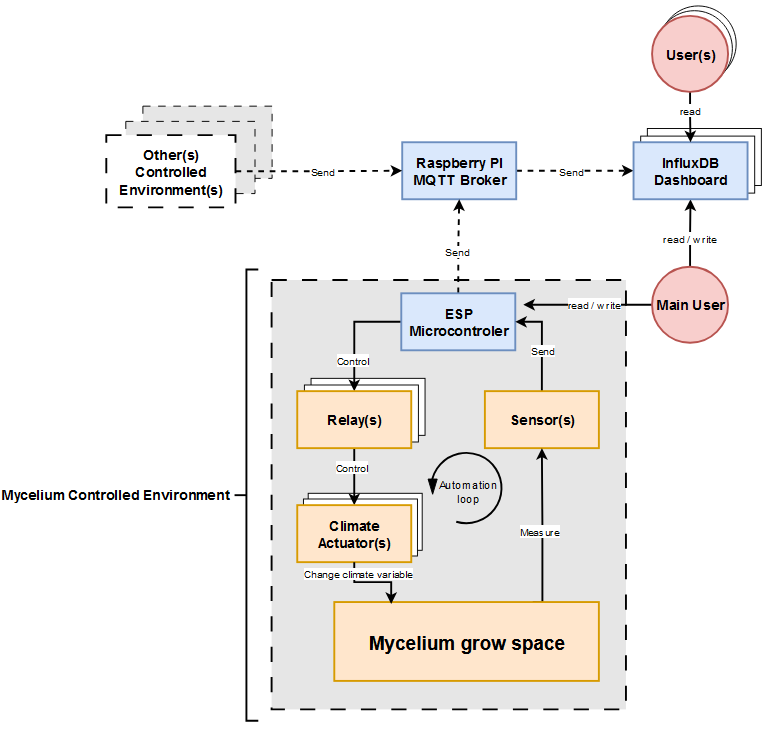
\includegraphics{images/diagMyceliummachine2.png}
    \caption{System design representation}
    \label{fig:blasttrash}
\end{figure} 


\section{Manufacturing Processes \& Grow Theory}

\section{Contribution}

\subsection{Environment controlled}
\subsection{Modular environmental control}



\section{Result}
\subsection{Mechanical test}






